% !TEX root = ../../main.tex


\begin{figure}[!htb]
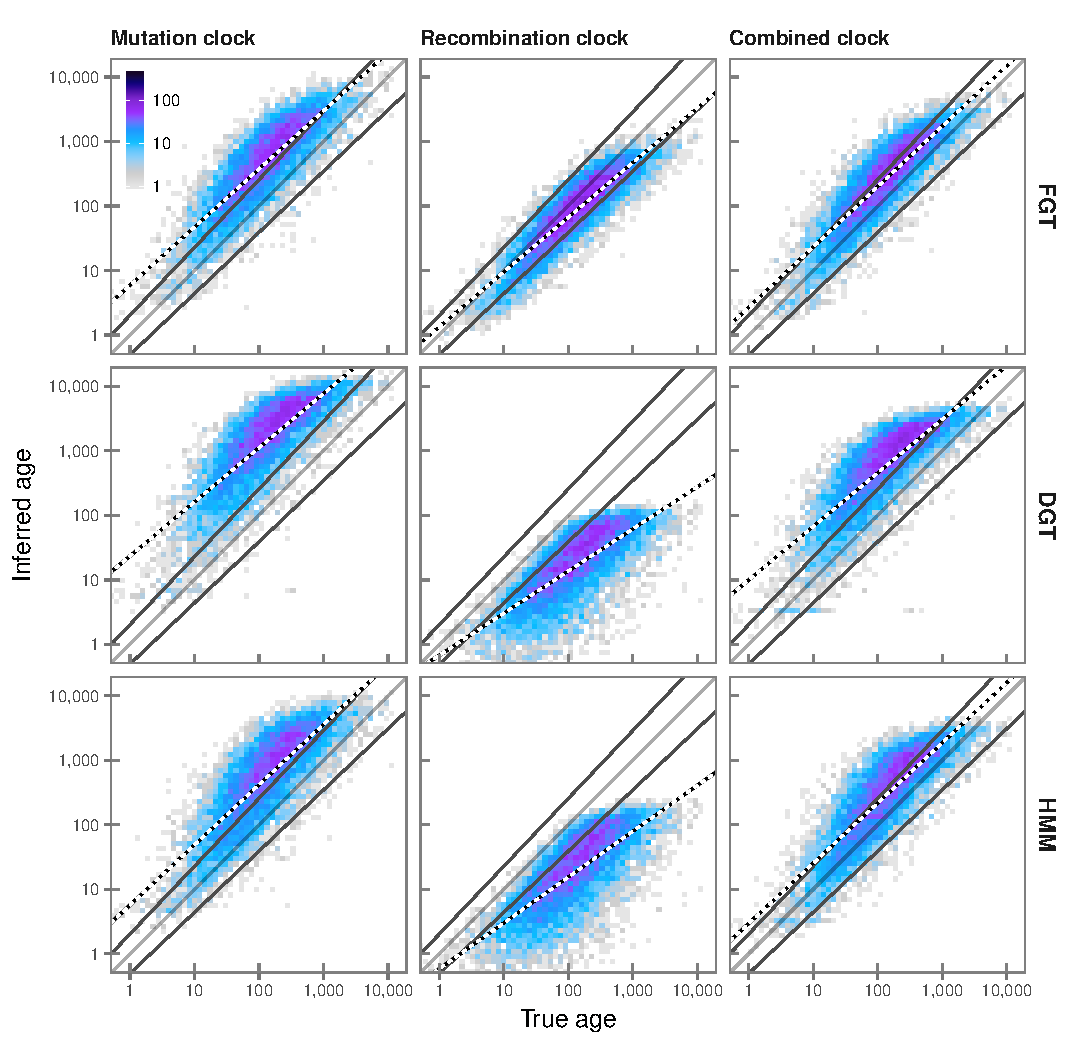
\includegraphics[width=\textwidth]{./img/ch5/vanilla_scat}
\Caption{Distribution of true and inferred age using different IBD detection methods}
{The \n{3} IBD detection methods \gls{fgt}, \gls{dgt}, and \gls{hmm} were compared under each clock model, on the same set of target sites that were drawn from \fk{[2,20]} variants (allele frequency ${\leq 1\%}$) in $\mathcal{D}_A$.
Each panel shows the density of true age ($t_m$) and inferred age.
Lines \emph{below} and \emph{above} the dividing line are regression trend lines of the corresponding true coalescent times around each mutation event, $t_c$ and $t_d$, respectively.
The regression of inferred age ($\hat{t}$) is given by the \emph{black-white} line.}
{fig:vanilla_scat}
\end{figure}
